\documentclass{article}
\usepackage[a4paper]{geometry}% just for the example
\usepackage[placment=top]{background}
\usepackage{draftwatermark}
\usepackage{tikz}
\backgroundsetup{%
  scale=0.8,            %% Size - change accordingly
  angle=0,              %% change accordingly
  opacity=0.4,          %% change accordingly
  color =black,         %% change accordingly
  position={10.7,-9.4}, %% change accordingly
  contents={\includegraphics[width=0.5\paperwidth,height=0.35\paperheight]{cycle.jpg}
    }%}    
    }
\begin{document}
\noindent

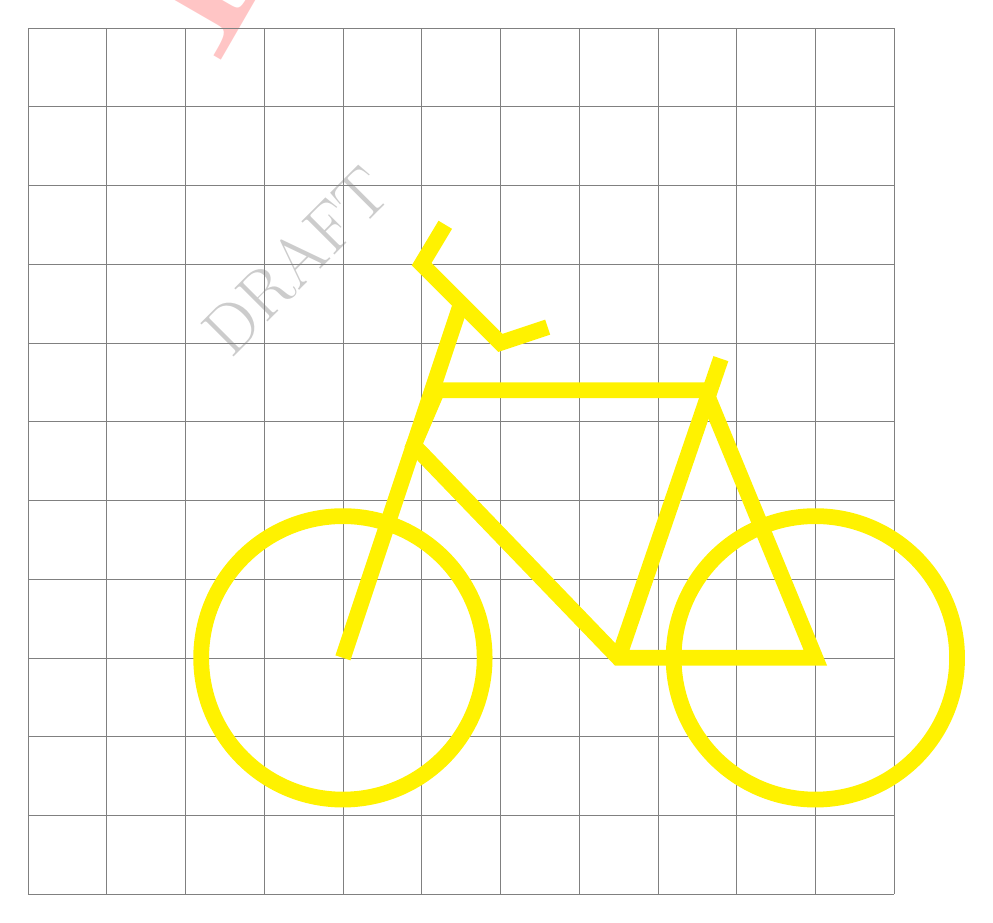
\begin{tikzpicture}[color=yellow,line width=2mm]
\draw[step=1cm,gray,very thin] (0,0) grid (11,11);
% origin (0,0) at bottom left
\draw (10,3) circle(1.8);
\draw (4,3) circle(1.8);
\draw (10,3) -- (8.6,6.4) -- (5.2,6.4) -- (4.9,5.7)
-- (7.5,3) --cycle;
\draw (7.5,3) -- (8.8,6.8);
\draw (4,3) -- (5.5,7.5);
\draw (5.3,8.5) -- (5,8) -- (6,7) -- (6.6,7.2);

\end{tikzpicture}
\end{document}